\chapter{Planificación}
\section[Diagrama de Gantt]{Diagrama de Gantt}
En esta sección se muestra una diagrama de Gantt con la planificación del proyecto dividido en diferentes tareas. La figura que contiene el diagrama \ref{fig:gantt} se encuentra al final de esta sección. Las tareas en las que se ha dividido el proyecto son las siguientes:
\begin{itemize}
	\item \textbf{Investigación sobre el problema:}
	\item \textbf{Investigación sobre herramientas para el desarrollo:}
	\item \textbf{Análisis de requisitos:}
	\item \textbf{Diseño:}
	\item \textbf{Implementación:}
	\item \textbf{Evaluación y pruebas:}
\end{itemize}

\section[Herramientas utilizadas para la planificación]{Herramientas utilizadas para la planificación}
\subsection{Trello}
\subsection{GitHub}

\begin{figure}[b]
	\centering
	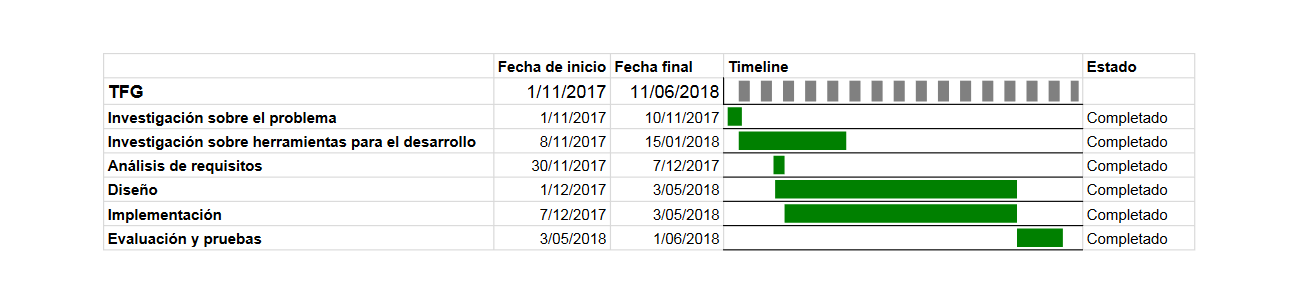
\includegraphics[scale=0.55,angle=90]{imagenes/Gantt.png}
	\caption{Planificación del proyecto}
	\label{fig:gantt}
\end{figure}
